\documentclass{article}
\usepackage[utf8]{inputenc}

\title{Project : Face and Digit Classification}
\author{James Wo, Rahul Patel }
\date{April 2020}

\usepackage{natbib}
\usepackage{graphicx}
\usepackage[parfill]{parskip}


\begin{document}

\maketitle

\section{Introduction}
For this project, we implemented three algorithms to deal with face and digit classification:
\begin{enumerate}
    \item Perceptron
    \item Naive Bayes Classifier
    \item K-Nearest Neighbors
\end{enumerate}
The following sections will describe these implemented algorithms as well as their results and learned lessons.

\section{Perceptron}
\\
\textbf{Description and Implementation:}

Given a feature list f, the perceptron calculates the class y whose weight vector is most similar to input vector f. For each iteration, we loop through the training data and compute the summation of weights multiplied by corresponding feature value. \\

\[
score(f,y) &= \sum_i f_i w_i^y
\]
\\
 We choose the label with the highest score as the predicted label for a particular data
 instance. \\ \\
 y' = arg max score(f, y'') \\ \\
 If predicted label (y') == true label (y), we have the correct instance and do nothing. Otherwise, we adjust the weights. w\textsuperscript{y} should have a higher f, and w\textsuperscript{y'} should have a lower f.  \\ \\
 if f(x\textsubscript{i}, w) \textless  0: \\
 w\textsuperscript{y} = w\textsuperscript{y} + f \\ \\
 if f(x\textsubscript{i}, w) \ge 0: \\
 w\textsuperscript{y'} = w\textsuperscript{y'} - f 
 \\ \\
 
If we include bias, there are minor adjustments to make. During summation, we have to include w\textsubscript{0} as the bias. Also, when adjusting weights, \\ w\textsubscript{0} = w\textsubscript{0} + 1 if f(x\textsubscript{i}, w) \textless  0 \\ \\ w\textsubscript{0} = w\textsubscript{0} - 1 if f(x\textsubscript{i}, w) \ge 0\\
 
\textbf{Results and Observations}:\\
\\

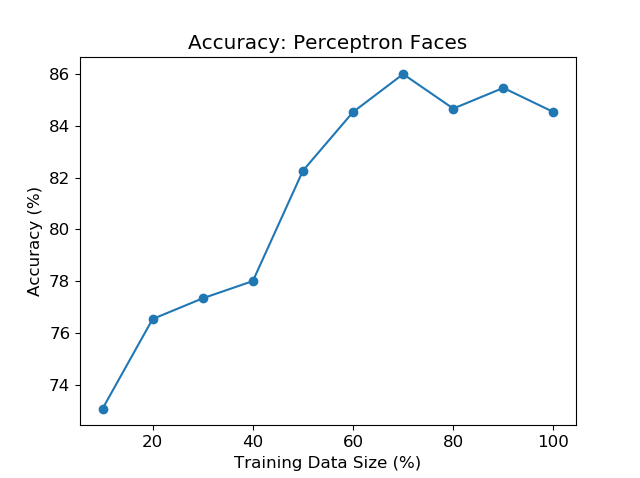
\includegraphics[width=0.8\textwidth,height=0.8\textheight,keepaspectratio]{p_f.png}

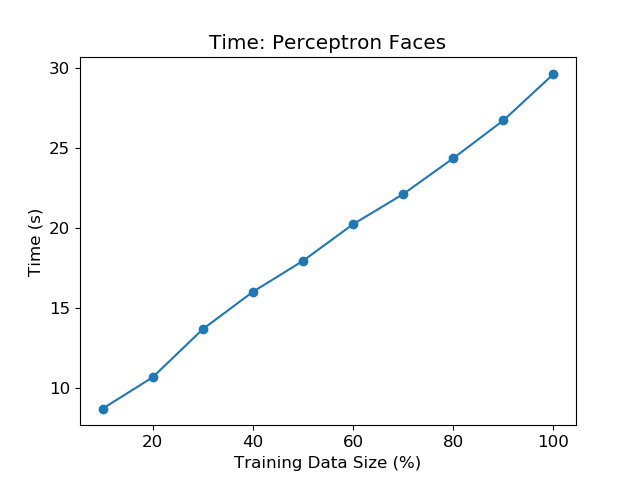
\includegraphics[width=0.8\textwidth,height=0.8\textheight,keepaspectratio]{p_f-t.png}

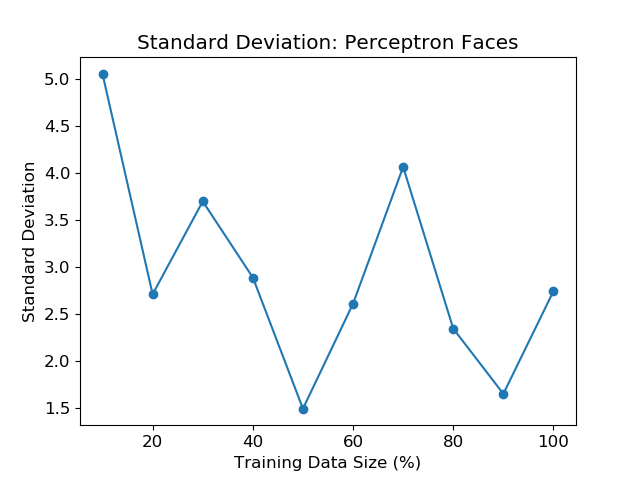
\includegraphics[width=0.8\textwidth,height=0.8\textheight,keepaspectratio]{std_pf.png}


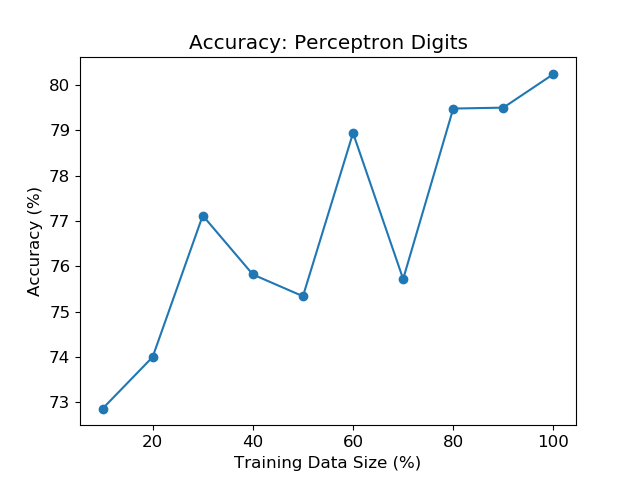
\includegraphics[width=0.8\textwidth,height=0.8\textheight,keepaspectratio]{p_d.png}

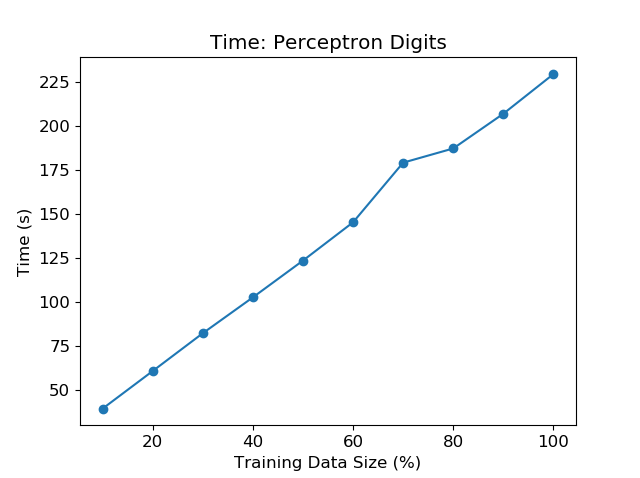
\includegraphics[width=0.8\textwidth,height=0.8\textheight,keepaspectratio]{p_d-t.png}
 
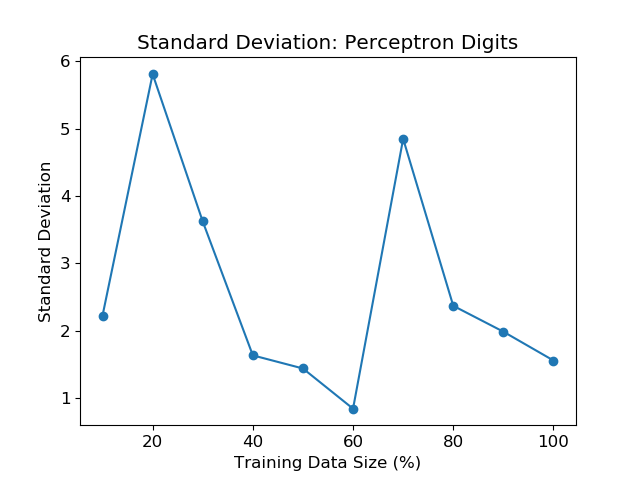
\includegraphics[width=0.8\textwidth,height=0.8\textheight,keepaspectratio]{std_pd.png}

What was notable for Perceptron was that it proved to be effective in classifying both digits and faces, as it surpassed 80\% accuracy in both cases. In both cases, we used the basic feature extraction, considering each pixel a binary feature. Although accuracy ultimately increased as training data size increased, the standard deviation for both classifications was very volatile throughout, relative to the other two algorithms. Interestingly enough, the standard deviation in accuracy for classifying digits was roughly the same for 10\% training data and 100\% training data.


\section{Naive Bayes Classifier}\\

\textbf{Description and Implementation:}

The Naive Bayes algorithm works upon Bayes Rule:\\
\\
\Pr(y \mid x) = \Pr(x \mid y)\Pr(y)/\Pr(x)\\

Before implementing Naive Bayes Classifier, we had to thoroughly understand this equation and its intuitions: \\

In the context of classification, the variable $y$ can be seen as the hidden variable. More specifically, it is the probability of a certain label. For the binary face classification, the variable $y$ can take on values $0$ and $1$, and for the digit classification, the variable $y$ can take on values $0$ to $9$. The variable $x$ is considered to be the evidence or data. The expression $\Pr(y \mid x)$ can thus be interpreted as the probability that an image can be classified as a certain label given the image's evidence or data. 
\\

Now, more importantly, observing the right side of the equation, we can treat $\Pr(y)$ as the initial, uninformed belief of the image, or how likely we think a certain label is for the image before seeing the image's evidence. This is contrasted with $\Pr(y \mid x)$, which is the informed belief of the image, or how likely we think a certain label is for the image after seeing the image's evidence. We then treat $\Pr(x \mid y)$ as how much the evidence $x$ supports the initial belief. In other words, assuming that our initial belief is correct, what were the chances that we see this image's evidence? 
\\

For a Naive Bayes Classifier, we would have to compute $\Pr(y \mid x)$ across all values of y (computing the probabilities of all possible labels of the image) and find the maximum probability and return the respective label. Because we only concern ourselves with the maximum probability, we only concern ourselves with the label with the largest $\Pr(x \mid Y=y)\Pr(Y=y)$ because the denominator, $\Pr(x)$ is constant because the image's evidence trivially stays the same as we consider different labels.
\\

The bulk of the programming for Naive Bayes Classifier was then to compute $\Pr(x \mid Y=y)\Pr(Y=y)$ (log joint probability) for all possible y for each image given. We knew that $\Pr(Y=y)$ is simply the probability of y in the training data. To find $\Pr(Y=y)$, I created a Counter object and traversed through the list of training labels given. For each label in the list, I incremented CounterA[label]. Thus, at the end of the traversal, this counter will have recorded the number of occurrences for each label in the training data. After this, I simply divided each value by size of the training labels list such that CounterA[label] will have the probability of seeing that label in the training data, or the initial beliefs, $\Pr(Y=y)$.
\\

For, $\Pr(x \mid Y=y)$, we knew $\Pr(x \mid Y=y) = \prod_{j=1}^{l}\Pr(\phi(x) \mid Y= y)$ =
$\prod_{j=1}^{l}X$ where $X =$ (Number of times $\phi(x) = v$ and $Y=y$ in training)/(Number of times $Y=y$ in training). Thus, to find $\Pr(x \mid Y=y)$, we first made a Counter object dedicated to count the number of times we see each feature (for each label) take on the value of 1 (We only used features that were either 1 or 0). We used a nested for loop that would go through every feature of every image and we would increment CounterB[(feature,label)] every time the current feature's value is 1. Thus, after visiting every image in the training set, CounterB[(feature,label)] would hold the number of training datum with the specific label where its value of the given feature is 1. After this, we divided every value in the counter by the number of occurrences of the given label, such that CounterB[(feature,label] would hold the probability $\Pr(\phi(x) = v \mid Y=y)$
\\

After populating these two counters, we wanted to find the log joint probability of $\Pr(x \mid Y=y)\Pr(Y=y)$ of a given image for each label (if we multiply like in Bayes rule it would result in too small of a value). First, we initialize the probability value to $\log (CounterA[label])$ Then, we would iterate through each feature of the given image. If the feature is 1, we would add the value $\log (Counter[(feature,label)])$ to the probability value. If the feature value is 0, we would add the value $\log (1-Counter[(feature,label)])$. At the end of the iteration, we have the complete log joint probability of a certain image for a given label and we would repeat the same process across the remaining labels.

Once we return the list of log joint probabilities across all the labels, the Berkeley skeleton picks the maximum accordingly.

\textbf{Results and Observations}:\\

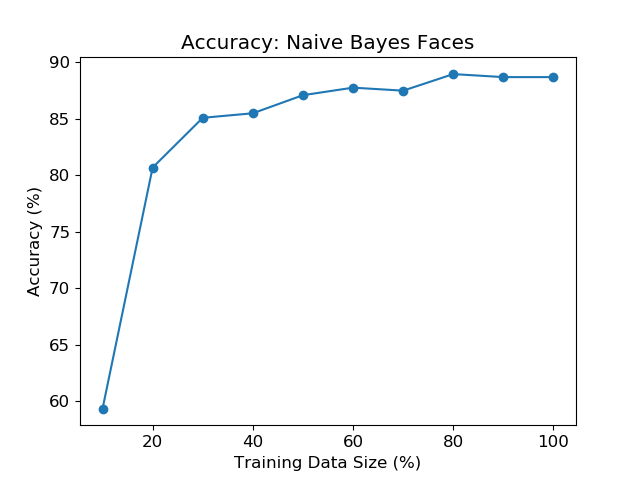
\includegraphics[width=0.8\textwidth,height=0.8\textheight,keepaspectratio]{n_f.png}

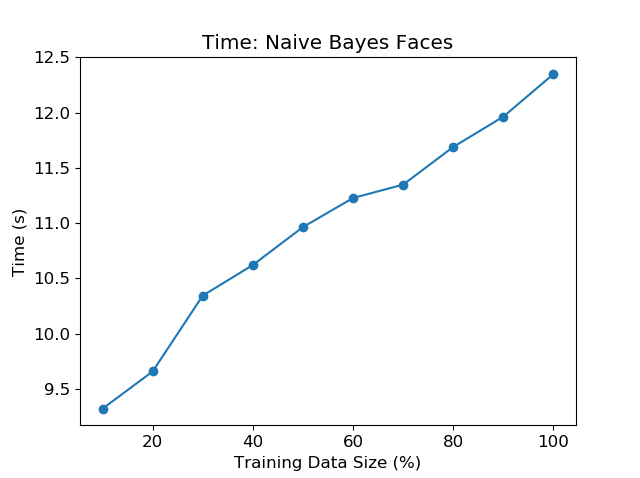
\includegraphics[width=0.8\textwidth,height=0.8\textheight,keepaspectratio]{n_f-t.png}

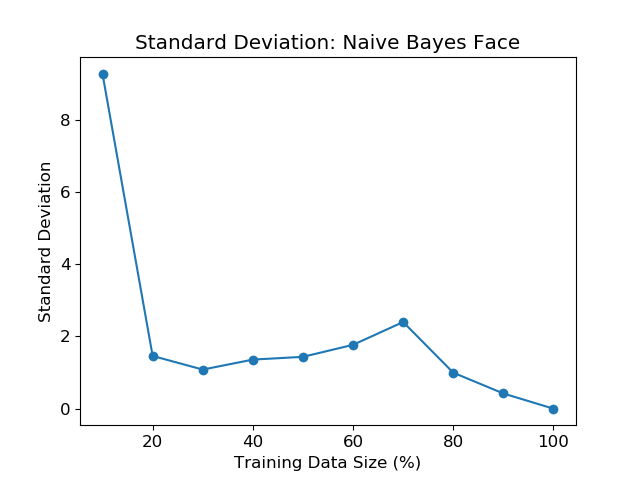
\includegraphics[width=0.8\textwidth,height=0.8\textheight,keepaspectratio]{std_nf.png}

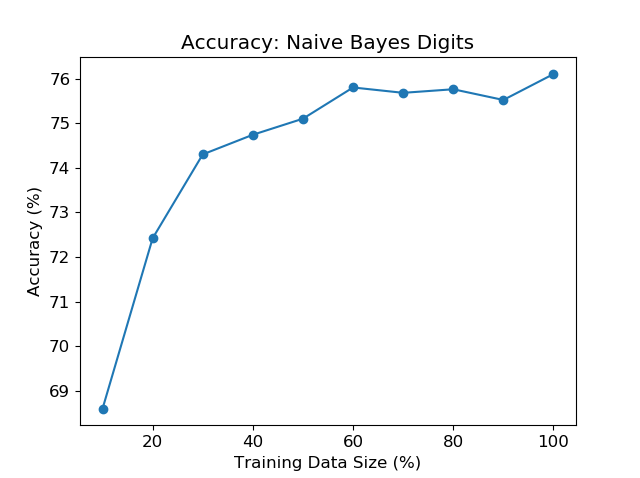
\includegraphics[width=0.8\textwidth,height=0.8\textheight,keepaspectratio]{n_d.png}

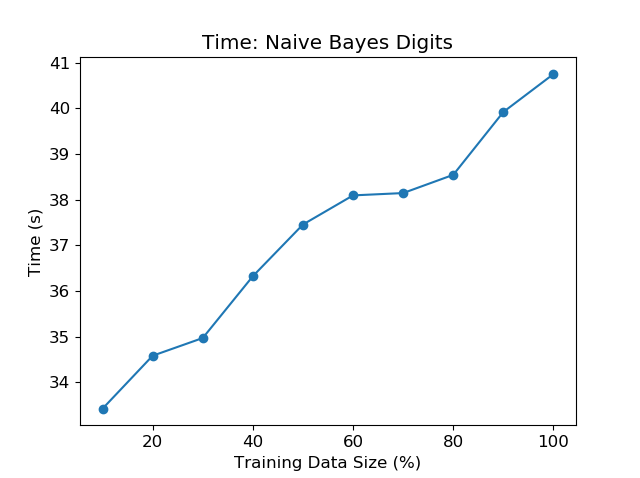
\includegraphics[width=0.8\textwidth,height=0.8\textheight,keepaspectratio]{n_d-t.png}\\

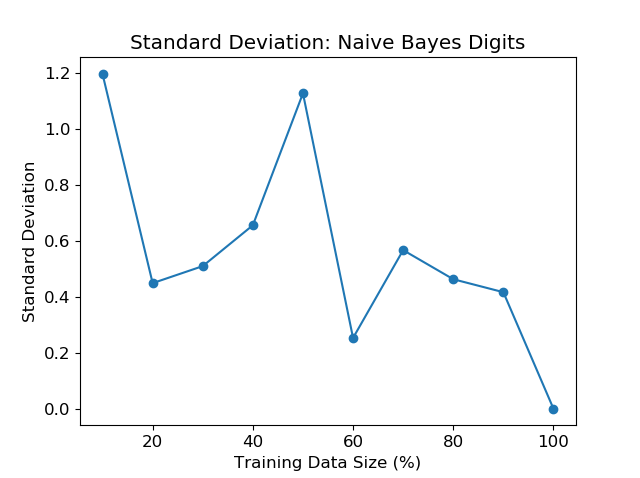
\includegraphics[width=0.8\textwidth,height=0.8\textheight,keepaspectratio]{std_nd.png}

Naive Bayes Classifier was fairly accurate in classifying faces, as its accuracy approached 90\% when using the entire data set.\\

For classifying digits, Naive Bayes still surpassed the 70\% requirement but did not do as well as it did for faces. Intuitively, this makes sense because dealing with digits involves dealing with more labels and probabilities.\\

What was interesting is that the learning in the beginning was much faster than learning later on. This contrasts with the relatively steady increase in learning for the perceptron algorithm (at least for faces). This can most likely be explained by Naive Bayes' complete reliance on training data. When the training data is small, it is likely the model has not seen all possible labels, and thus heavily penalizes testing datum that has a label it has not seen. This results in poor accuracy. Once it is able to see all labels, its accuracy would increase drastically. 


\section{K-Nearest Neighbors}\\

\textbf{Description and Implementation:}

The K-Nearest Neighbors algorithm plots each training datum on an n dimensional graph, where there are n features specified. It simply classifies each testing datum by plotting it on the same graph, and observing the k closest training datum points to it. Amongst those k closest points, the label that occurs the most frequent will be the label assigned to the testing datum.\\

We first started by creating two lists of Numpy arrays, one for the training data and one for the testing data. Each Numpy array in the list would represent a training/testing datum's features. Because our feature values are binary, there is a Numpy array of 0's and 1's for each datum. We then created a nested for loop: for each testing datum in the list, we would visit each training datum and find the distance between them and append it to a distance array. Thus, after visiting each training datum, the distance array holds how far every training datum is to the test datum. Because our k constant is set to 3, we sort the array and store the 3 indices of the 3 closest training datum in an indices array. Afterwards, we iterate through the indices array and keep tally (with a counter object) of the occurrences of each label (we use the indices to index into the training label list to see which labels the 3 closest training datum corresponded to). We return the label that occurs the most frequent.\\

\textbf{Results and Observations}:\\

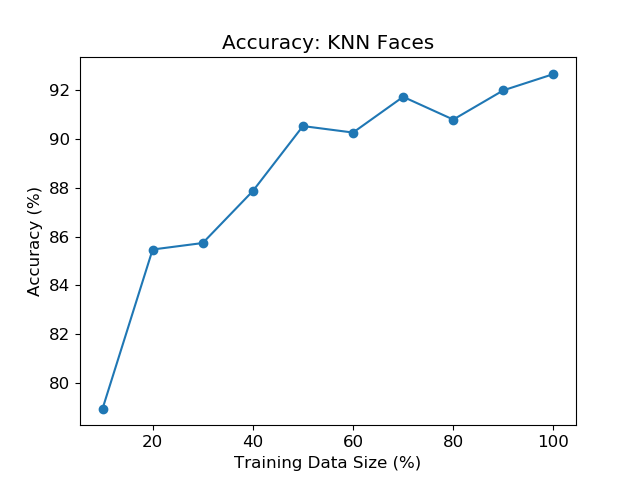
\includegraphics[width=0.8\textwidth,height=0.8\textheight,keepaspectratio]{k_f.png}

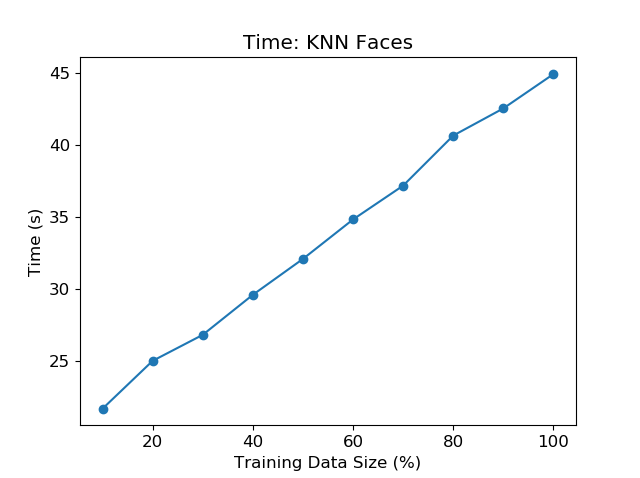
\includegraphics[width=0.8\textwidth,height=0.8\textheight,keepaspectratio]{k_f-t.png}

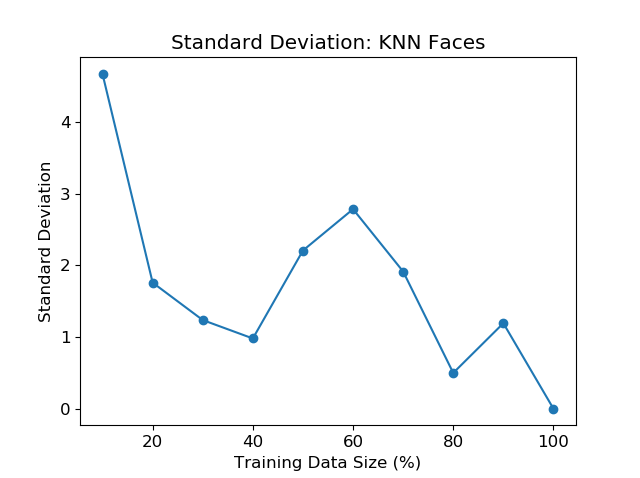
\includegraphics[width=0.8\textwidth,height=0.8\textheight,keepaspectratio]{std_kf.png}

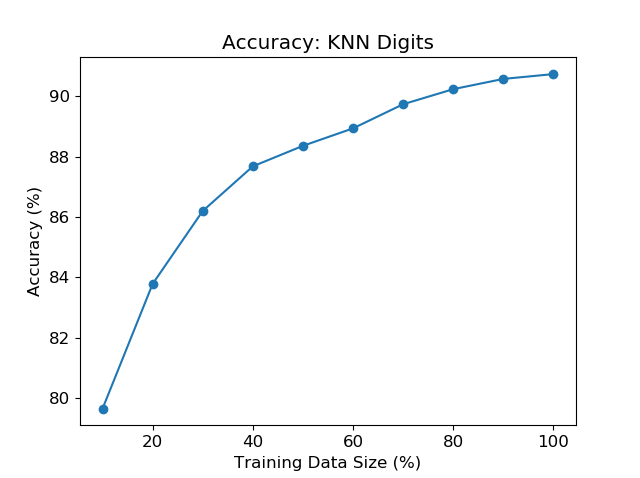
\includegraphics[width=0.8\textwidth,height=0.8\textheight,keepaspectratio]{k_d.png}

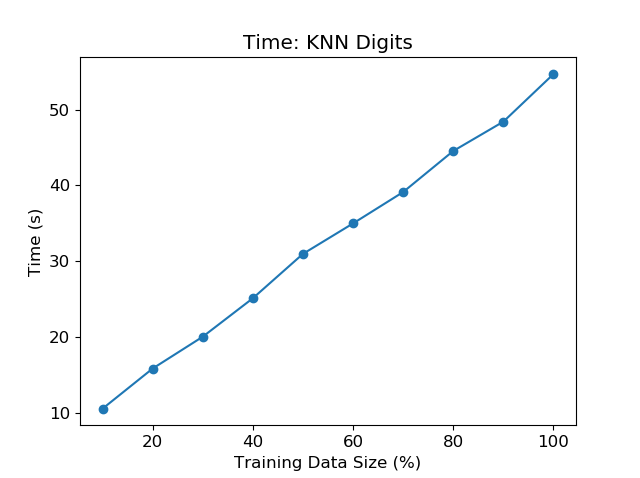
\includegraphics[width=0.8\textwidth,height=0.8\textheight,keepaspectratio]{k_d-t.png}

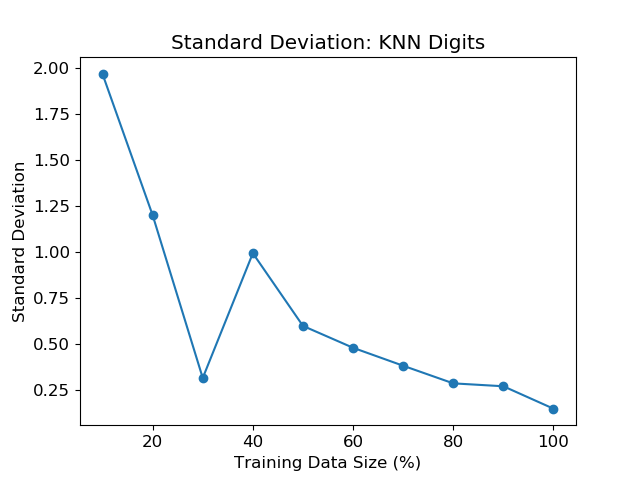
\includegraphics[width=0.8\textwidth,height=0.8\textheight,keepaspectratio]{std_kd.png}

We observed that K-Nearest Neighbors algorithm was very effective for classifying digits when using the basic features (1 pixel is 1 feature) as the accuracy surpassed 90\% and its standard deviation approached 0. In fact, it seems like KNN did the best out of the three algorithms for digit classification.

However, in order to reach the 70\% accuracy requirement when classifying faces, we had to resort to enhanced features (single gradient feature extraction) because using the basic features yielded poor results. This was the only time we had to use enhanced feature extraction; This at first seemed counter-intuitive to us because it seems that classifying digits is a more difficult job to do accurately than classifying faces, as there are more labels to consider. We propose the following explanation: KNN works best when there are isolated clusters of training datum for each label. The basic features for faces most likely do not allow for more isolated clusters and thus makes classifying less accurate. The nature of the data images of faces may also seem to play a role - perhaps the euclidean distance between "face" and "not face" is smaller than the euclidean distance between different digits, thus requiring a more advanced feature extraction technique for accuracy to be good. The less distinct differences for face classification would also explain the KNN's volatile standard deviation for face classification. \\

As training data size increased, KNN classification accuracy steadily increased for both types. This makes sense as KNN's "training" is wholly dependent on the training data, similar to the Naive Bayes classifier. As more data is given to the model, the more accurately it can discern labels and clusters. \\




\section{Additional Comparisons}\\
Although almost all three algorithms exhibited linear growth for time taken to train, perceptron took significantly more time than the other two. This is most likely due to the computationally heavy readjustments of weights and the multiple iterations. When KNN and Naive Bayes trains, they are simply storing/counting through the training data, which is much less demanding.\\

Naive Bayes seems to have yielded the worst accuracy for classifying digits. This can most likely be attributed to the assumption that Naive Bayes makes - that all features are independent of another. Of course, for numbers, this seems to be an inaccurate assumption since certain traits of a number's image can be dependent on other traits. \\


\section{Closing Remarks}
Overall, it was very enlightening to witness relatively simple algorithms learn and classify fairly well. It was also interesting to see how computationally demanding some algorithms turned out to be when the training/data set size increased. 

\end{document}
